% Options for packages loaded elsewhere
% Options for packages loaded elsewhere
\PassOptionsToPackage{unicode}{hyperref}
\PassOptionsToPackage{hyphens}{url}
\PassOptionsToPackage{dvipsnames,svgnames,x11names}{xcolor}
%
\documentclass[
  spanish,
  11pt,
  a4paper,
  DIV=11,
  numbers=noendperiod]{scrartcl}
\usepackage{xcolor}
\usepackage[margin=2.5cm]{geometry}
\usepackage{amsmath,amssymb}
\setcounter{secnumdepth}{5}
\usepackage{iftex}
\ifPDFTeX
  \usepackage[T1]{fontenc}
  \usepackage[utf8]{inputenc}
  \usepackage{textcomp} % provide euro and other symbols
\else % if luatex or xetex
  \usepackage{unicode-math} % this also loads fontspec
  \defaultfontfeatures{Scale=MatchLowercase}
  \defaultfontfeatures[\rmfamily]{Ligatures=TeX,Scale=1}
\fi
\usepackage{lmodern}
\ifPDFTeX\else
  % xetex/luatex font selection
  \setmainfont[]{Times New Roman}
\fi
% Use upquote if available, for straight quotes in verbatim environments
\IfFileExists{upquote.sty}{\usepackage{upquote}}{}
\IfFileExists{microtype.sty}{% use microtype if available
  \usepackage[]{microtype}
  \UseMicrotypeSet[protrusion]{basicmath} % disable protrusion for tt fonts
}{}
\makeatletter
\@ifundefined{KOMAClassName}{% if non-KOMA class
  \IfFileExists{parskip.sty}{%
    \usepackage{parskip}
  }{% else
    \setlength{\parindent}{0pt}
    \setlength{\parskip}{6pt plus 2pt minus 1pt}}
}{% if KOMA class
  \KOMAoptions{parskip=half}}
\makeatother
% Make \paragraph and \subparagraph free-standing
\makeatletter
\ifx\paragraph\undefined\else
  \let\oldparagraph\paragraph
  \renewcommand{\paragraph}{
    \@ifstar
      \xxxParagraphStar
      \xxxParagraphNoStar
  }
  \newcommand{\xxxParagraphStar}[1]{\oldparagraph*{#1}\mbox{}}
  \newcommand{\xxxParagraphNoStar}[1]{\oldparagraph{#1}\mbox{}}
\fi
\ifx\subparagraph\undefined\else
  \let\oldsubparagraph\subparagraph
  \renewcommand{\subparagraph}{
    \@ifstar
      \xxxSubParagraphStar
      \xxxSubParagraphNoStar
  }
  \newcommand{\xxxSubParagraphStar}[1]{\oldsubparagraph*{#1}\mbox{}}
  \newcommand{\xxxSubParagraphNoStar}[1]{\oldsubparagraph{#1}\mbox{}}
\fi
\makeatother

\usepackage{color}
\usepackage{fancyvrb}
\newcommand{\VerbBar}{|}
\newcommand{\VERB}{\Verb[commandchars=\\\{\}]}
\DefineVerbatimEnvironment{Highlighting}{Verbatim}{commandchars=\\\{\}}
% Add ',fontsize=\small' for more characters per line
\usepackage{framed}
\definecolor{shadecolor}{RGB}{241,243,245}
\newenvironment{Shaded}{\begin{snugshade}}{\end{snugshade}}
\newcommand{\AlertTok}[1]{\textcolor[rgb]{0.68,0.00,0.00}{#1}}
\newcommand{\AnnotationTok}[1]{\textcolor[rgb]{0.37,0.37,0.37}{#1}}
\newcommand{\AttributeTok}[1]{\textcolor[rgb]{0.40,0.45,0.13}{#1}}
\newcommand{\BaseNTok}[1]{\textcolor[rgb]{0.68,0.00,0.00}{#1}}
\newcommand{\BuiltInTok}[1]{\textcolor[rgb]{0.00,0.23,0.31}{#1}}
\newcommand{\CharTok}[1]{\textcolor[rgb]{0.13,0.47,0.30}{#1}}
\newcommand{\CommentTok}[1]{\textcolor[rgb]{0.37,0.37,0.37}{#1}}
\newcommand{\CommentVarTok}[1]{\textcolor[rgb]{0.37,0.37,0.37}{\textit{#1}}}
\newcommand{\ConstantTok}[1]{\textcolor[rgb]{0.56,0.35,0.01}{#1}}
\newcommand{\ControlFlowTok}[1]{\textcolor[rgb]{0.00,0.23,0.31}{\textbf{#1}}}
\newcommand{\DataTypeTok}[1]{\textcolor[rgb]{0.68,0.00,0.00}{#1}}
\newcommand{\DecValTok}[1]{\textcolor[rgb]{0.68,0.00,0.00}{#1}}
\newcommand{\DocumentationTok}[1]{\textcolor[rgb]{0.37,0.37,0.37}{\textit{#1}}}
\newcommand{\ErrorTok}[1]{\textcolor[rgb]{0.68,0.00,0.00}{#1}}
\newcommand{\ExtensionTok}[1]{\textcolor[rgb]{0.00,0.23,0.31}{#1}}
\newcommand{\FloatTok}[1]{\textcolor[rgb]{0.68,0.00,0.00}{#1}}
\newcommand{\FunctionTok}[1]{\textcolor[rgb]{0.28,0.35,0.67}{#1}}
\newcommand{\ImportTok}[1]{\textcolor[rgb]{0.00,0.46,0.62}{#1}}
\newcommand{\InformationTok}[1]{\textcolor[rgb]{0.37,0.37,0.37}{#1}}
\newcommand{\KeywordTok}[1]{\textcolor[rgb]{0.00,0.23,0.31}{\textbf{#1}}}
\newcommand{\NormalTok}[1]{\textcolor[rgb]{0.00,0.23,0.31}{#1}}
\newcommand{\OperatorTok}[1]{\textcolor[rgb]{0.37,0.37,0.37}{#1}}
\newcommand{\OtherTok}[1]{\textcolor[rgb]{0.00,0.23,0.31}{#1}}
\newcommand{\PreprocessorTok}[1]{\textcolor[rgb]{0.68,0.00,0.00}{#1}}
\newcommand{\RegionMarkerTok}[1]{\textcolor[rgb]{0.00,0.23,0.31}{#1}}
\newcommand{\SpecialCharTok}[1]{\textcolor[rgb]{0.37,0.37,0.37}{#1}}
\newcommand{\SpecialStringTok}[1]{\textcolor[rgb]{0.13,0.47,0.30}{#1}}
\newcommand{\StringTok}[1]{\textcolor[rgb]{0.13,0.47,0.30}{#1}}
\newcommand{\VariableTok}[1]{\textcolor[rgb]{0.07,0.07,0.07}{#1}}
\newcommand{\VerbatimStringTok}[1]{\textcolor[rgb]{0.13,0.47,0.30}{#1}}
\newcommand{\WarningTok}[1]{\textcolor[rgb]{0.37,0.37,0.37}{\textit{#1}}}

\usepackage{longtable,booktabs,array}
\usepackage{calc} % for calculating minipage widths
% Correct order of tables after \paragraph or \subparagraph
\usepackage{etoolbox}
\makeatletter
\patchcmd\longtable{\par}{\if@noskipsec\mbox{}\fi\par}{}{}
\makeatother
% Allow footnotes in longtable head/foot
\IfFileExists{footnotehyper.sty}{\usepackage{footnotehyper}}{\usepackage{footnote}}
\makesavenoteenv{longtable}
\usepackage{graphicx}
\makeatletter
\newsavebox\pandoc@box
\newcommand*\pandocbounded[1]{% scales image to fit in text height/width
  \sbox\pandoc@box{#1}%
  \Gscale@div\@tempa{\textheight}{\dimexpr\ht\pandoc@box+\dp\pandoc@box\relax}%
  \Gscale@div\@tempb{\linewidth}{\wd\pandoc@box}%
  \ifdim\@tempb\p@<\@tempa\p@\let\@tempa\@tempb\fi% select the smaller of both
  \ifdim\@tempa\p@<\p@\scalebox{\@tempa}{\usebox\pandoc@box}%
  \else\usebox{\pandoc@box}%
  \fi%
}
% Set default figure placement to htbp
\def\fps@figure{htbp}
\makeatother



\ifLuaTeX
\usepackage[bidi=basic]{babel}
\else
\usepackage[bidi=default]{babel}
\fi
\ifPDFTeX
\else
\babelfont{rm}[]{Times New Roman}
\fi
% get rid of language-specific shorthands (see #6817):
\let\LanguageShortHands\languageshorthands
\def\languageshorthands#1{}


\setlength{\emergencystretch}{3em} % prevent overfull lines

\providecommand{\tightlist}{%
  \setlength{\itemsep}{0pt}\setlength{\parskip}{0pt}}



 


\KOMAoption{captions}{tableheading}
\makeatletter
\@ifpackageloaded{caption}{}{\usepackage{caption}}
\AtBeginDocument{%
\ifdefined\contentsname
  \renewcommand*\contentsname{Tabla de contenidos}
\else
  \newcommand\contentsname{Tabla de contenidos}
\fi
\ifdefined\listfigurename
  \renewcommand*\listfigurename{Listado de Figuras}
\else
  \newcommand\listfigurename{Listado de Figuras}
\fi
\ifdefined\listtablename
  \renewcommand*\listtablename{Listado de Tablas}
\else
  \newcommand\listtablename{Listado de Tablas}
\fi
\ifdefined\figurename
  \renewcommand*\figurename{Figura}
\else
  \newcommand\figurename{Figura}
\fi
\ifdefined\tablename
  \renewcommand*\tablename{Tabla}
\else
  \newcommand\tablename{Tabla}
\fi
}
\@ifpackageloaded{float}{}{\usepackage{float}}
\floatstyle{ruled}
\@ifundefined{c@chapter}{\newfloat{codelisting}{h}{lop}}{\newfloat{codelisting}{h}{lop}[chapter]}
\floatname{codelisting}{Listado}
\newcommand*\listoflistings{\listof{codelisting}{Listado de Listados}}
\makeatother
\makeatletter
\makeatother
\makeatletter
\@ifpackageloaded{caption}{}{\usepackage{caption}}
\@ifpackageloaded{subcaption}{}{\usepackage{subcaption}}
\makeatother
\usepackage{bookmark}
\IfFileExists{xurl.sty}{\usepackage{xurl}}{} % add URL line breaks if available
\urlstyle{same}
\hypersetup{
  pdftitle={Regresiones lineales simples y múltiples},
  pdfauthor={Santos G},
  pdflang={es},
  colorlinks=true,
  linkcolor={blue},
  filecolor={Maroon},
  citecolor={Blue},
  urlcolor={Blue},
  pdfcreator={LaTeX via pandoc}}


\title{Regresiones lineales simples y múltiples}
\author{Santos G}
\date{}
\begin{document}
\maketitle

\renewcommand*\contentsname{Tabla de contenidos}
{
\hypersetup{linkcolor=}
\setcounter{tocdepth}{2}
\tableofcontents
}

\section{Contexto de proyecto}\label{contexto-de-proyecto}

En esta sección se explora la relación entre variables morfológicas de
los pingüinos, en particular entre la longitud del ala (flipper length)
y la longitud del pico (bill length). El objetivo es evaluar si existe
una asociación lineal entre ambas medidas, lo que permitiría inferir
patrones de covariación corporal. Para ello, se aplican métodos de
regresión lineal, que asumen una relación lineal y aditiva entre las
variables, junto con verificaciones de supuestos estadísticos y
exploración de posibles valores atípicos o influyentes.

\section{Carga de librerías, dataset y limpieza de los
datos}\label{carga-de-libreruxedas-dataset-y-limpieza-de-los-datos}

\begin{Shaded}
\begin{Highlighting}[numbers=left,,]
\CommentTok{\# Cargar librerías}
\FunctionTok{library}\NormalTok{(tidyverse)    }\CommentTok{\# manipulación de datos y ggplot2}
\FunctionTok{library}\NormalTok{(palmerpenguins) }\CommentTok{\# dataset de pingüinos}
\FunctionTok{library}\NormalTok{(janitor)      }\CommentTok{\# limpieza de nombres de columnas}
\FunctionTok{library}\NormalTok{(broom)        }\CommentTok{\# resultados ordenados de modelos}
\FunctionTok{library}\NormalTok{(car)          }\CommentTok{\# pruebas estadísticas (ej. Levene)}

\CommentTok{\# Cargar dataset}
\NormalTok{df\_raw }\OtherTok{\textless{}{-}}\NormalTok{ penguins }\SpecialCharTok{\%\textgreater{}\%} \FunctionTok{as\_tibble}\NormalTok{() }\CommentTok{\# guardo raw para auditoría}
\NormalTok{df }\OtherTok{\textless{}{-}}\NormalTok{ df\_raw }\SpecialCharTok{\%\textgreater{}\%} \FunctionTok{clean\_names}\NormalTok{()}
\end{Highlighting}
\end{Shaded}

\section{Visualización inicial +
correlación}\label{visualizaciuxf3n-inicial-correlaciuxf3n}

\begin{Shaded}
\begin{Highlighting}[numbers=left,,]
\CommentTok{\# Scatter con línea de regresión (usa df ya limpio)}
\FunctionTok{ggplot}\NormalTok{(df, }\FunctionTok{aes}\NormalTok{(}\AttributeTok{x =}\NormalTok{ flipper\_length\_mm, }\AttributeTok{y =}\NormalTok{ bill\_length\_mm)) }\SpecialCharTok{+}
  \FunctionTok{geom\_point}\NormalTok{(}\AttributeTok{alpha =} \FloatTok{0.6}\NormalTok{) }\SpecialCharTok{+}
  \FunctionTok{geom\_smooth}\NormalTok{(}\AttributeTok{method =} \StringTok{"lm"}\NormalTok{, }\AttributeTok{se =} \ConstantTok{TRUE}\NormalTok{, }\AttributeTok{formula =}\NormalTok{ y }\SpecialCharTok{\textasciitilde{}}\NormalTok{ x) }\SpecialCharTok{+}
  \FunctionTok{labs}\NormalTok{(}\AttributeTok{x =} \StringTok{"Flipper length (mm)"}\NormalTok{, }\AttributeTok{y =} \StringTok{"Bill length (mm)"}\NormalTok{,}
       \AttributeTok{title =} \StringTok{"Relación bill\_length\_mm \textasciitilde{} flipper\_length\_mm"}\NormalTok{) }\SpecialCharTok{+}
  \FunctionTok{theme\_minimal}\NormalTok{()}
\end{Highlighting}
\end{Shaded}

\begin{figure}[H]

{\centering \pandocbounded{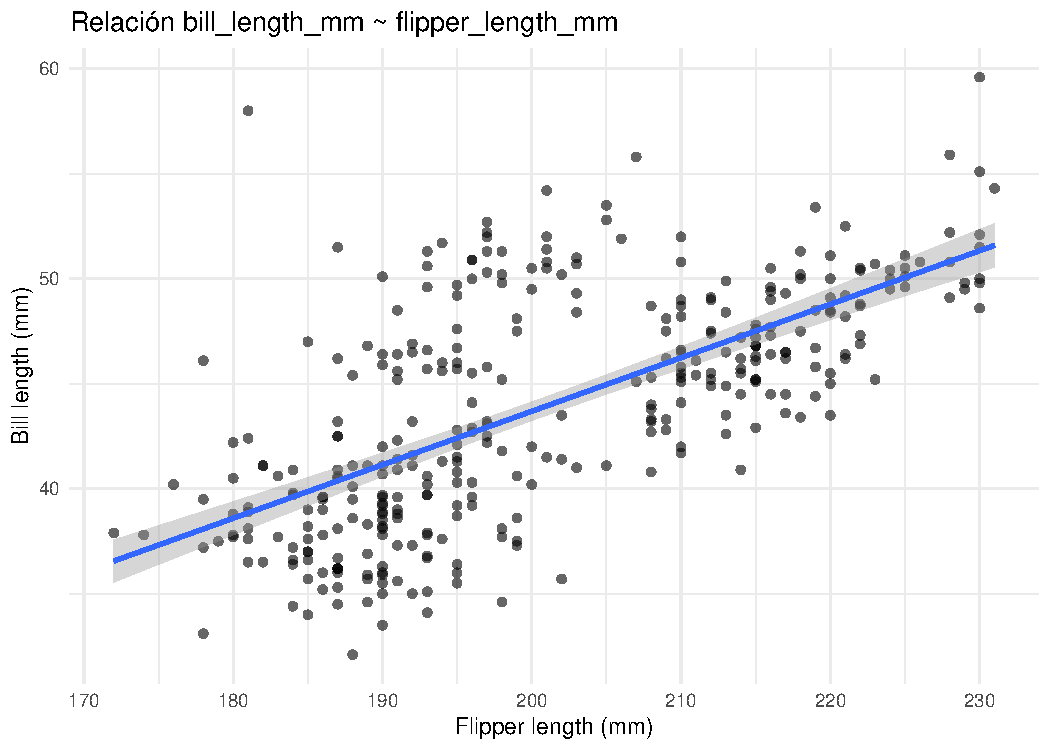
\includegraphics[keepaspectratio]{Regresiones-y-GLM_files/figure-pdf/scatter_cor-1.pdf}}

}

\caption{Scatter con línea de regresión entre las variables biil length
y flipper length.}

\end{figure}%

La \textbf{Figura 1} muestra una tendencia positiva clara: a mayor
longitud del ala (flipper length), mayor longitud del pico (bill
length). La nube de puntos es relativamente compacta, lo que sugiere una
asociación consistente entre ambas variables.

\begin{Shaded}
\begin{Highlighting}[numbers=left,,]
\CommentTok{\# Correlación Pearson y Spearman (devuelven objetos htest)}
\NormalTok{cor\_pearson }\OtherTok{\textless{}{-}} \FunctionTok{cor.test}\NormalTok{(df}\SpecialCharTok{$}\NormalTok{flipper\_length\_mm, df}\SpecialCharTok{$}\NormalTok{bill\_length\_mm, }
                        \AttributeTok{method =} \StringTok{"pearson"}\NormalTok{)}
\NormalTok{cor\_spearman }\OtherTok{\textless{}{-}} \FunctionTok{cor.test}\NormalTok{(df}\SpecialCharTok{$}\NormalTok{flipper\_length\_mm, df}\SpecialCharTok{$}\NormalTok{bill\_length\_mm, }
                         \AttributeTok{method =} \StringTok{"spearman"}\NormalTok{)}
\CommentTok{\# Correlación Pearson}
\NormalTok{pearson\_tab }\OtherTok{\textless{}{-}}\NormalTok{ broom}\SpecialCharTok{::}\FunctionTok{tidy}\NormalTok{(cor\_pearson) }\SpecialCharTok{\%\textgreater{}\%}
  \FunctionTok{select}\NormalTok{(estimate, statistic, p.value, conf.low, conf.high) }\SpecialCharTok{\%\textgreater{}\%}
  \FunctionTok{mutate}\NormalTok{(}
    \AttributeTok{p.value =} \FunctionTok{ifelse}\NormalTok{(p.value }\SpecialCharTok{\textless{}} \FloatTok{0.001}\NormalTok{, }\StringTok{"\textless{} 0.001"}\NormalTok{, }\FunctionTok{round}\NormalTok{(p.value, }\DecValTok{3}\NormalTok{)),}
    \FunctionTok{across}\NormalTok{(}\FunctionTok{where}\NormalTok{(is.numeric), round, }\DecValTok{3}\NormalTok{)}
\NormalTok{  )}

\NormalTok{knitr}\SpecialCharTok{::}\FunctionTok{kable}\NormalTok{(pearson\_tab, }\AttributeTok{caption =} \StringTok{"Correlación de Pearson }
\StringTok{             entre bill\_length y flipper\_length"}\NormalTok{)}
\end{Highlighting}
\end{Shaded}

\begin{longtable}[]{@{}rrlrr@{}}
\caption{Correlación de Pearson entre bill\_length y
flipper\_length}\tabularnewline
\toprule\noalign{}
estimate & statistic & p.value & conf.low & conf.high \\
\midrule\noalign{}
\endfirsthead
\toprule\noalign{}
estimate & statistic & p.value & conf.low & conf.high \\
\midrule\noalign{}
\endhead
\bottomrule\noalign{}
\endlastfoot
0.656 & 16.034 & \textless{} 0.001 & 0.591 & 0.713 \\
\end{longtable}

\begin{Shaded}
\begin{Highlighting}[numbers=left,,]
\CommentTok{\# Correlación Spearman}
\NormalTok{spearman\_tab }\OtherTok{\textless{}{-}}\NormalTok{ broom}\SpecialCharTok{::}\FunctionTok{tidy}\NormalTok{(cor\_spearman) }\SpecialCharTok{\%\textgreater{}\%}
  \FunctionTok{select}\NormalTok{(estimate, statistic, p.value) }\SpecialCharTok{\%\textgreater{}\%}
  \FunctionTok{mutate}\NormalTok{(}
    \AttributeTok{p.value =} \FunctionTok{ifelse}\NormalTok{(p.value }\SpecialCharTok{\textless{}} \FloatTok{0.001}\NormalTok{, }\StringTok{"\textless{} 0.001"}\NormalTok{, }\FunctionTok{round}\NormalTok{(p.value, }\DecValTok{3}\NormalTok{)),}
    \FunctionTok{across}\NormalTok{(}\FunctionTok{where}\NormalTok{(is.numeric), round, }\DecValTok{3}\NormalTok{)}
\NormalTok{  )}

\NormalTok{knitr}\SpecialCharTok{::}\FunctionTok{kable}\NormalTok{(spearman\_tab, }\AttributeTok{caption =} \StringTok{"Correlación de Spearman }
\StringTok{             entre bill\_length y flipper\_length"}\NormalTok{)}
\end{Highlighting}
\end{Shaded}

\begin{longtable}[]{@{}rrl@{}}
\caption{Correlación de Spearman entre bill\_length y
flipper\_length}\tabularnewline
\toprule\noalign{}
estimate & statistic & p.value \\
\midrule\noalign{}
\endfirsthead
\toprule\noalign{}
estimate & statistic & p.value \\
\midrule\noalign{}
\endhead
\bottomrule\noalign{}
\endlastfoot
0.673 & 2181594 & \textless{} 0.001 \\
\end{longtable}

Las \textbf{Tablas 1} y \textbf{2} reflejan que tanto el coeficiente de
Pearson (r = 0.656, p \textless{} 0.001) como el de Spearman (ρ = 0.673,
p \textless{} 0.001) confirman una correlación positiva, de magnitud
moderada a fuerte. Esto indica que el tamaño del pico está relacionado
con el tamaño corporal de los pingüinos, lo cual es esperado en términos
de allometría: individuos con alas más largas (indicador del tamaño
total) tienden a presentar picos más largos.

\section{Regresión lineal simple}\label{regresiuxf3n-lineal-simple}

\begin{Shaded}
\begin{Highlighting}[numbers=left,,]
\CommentTok{\# Ajuste del modelo lineal simple}
\NormalTok{modelo\_lm }\OtherTok{\textless{}{-}} \FunctionTok{lm}\NormalTok{(bill\_length\_mm }\SpecialCharTok{\textasciitilde{}}\NormalTok{ flipper\_length\_mm, }\AttributeTok{data =}\NormalTok{ df)}

\CommentTok{\# Coeficientes y resumen del ajuste}
\NormalTok{tidy\_lm }\OtherTok{\textless{}{-}}\NormalTok{ broom}\SpecialCharTok{::}\FunctionTok{tidy}\NormalTok{(modelo\_lm)}
\NormalTok{glance\_lm }\OtherTok{\textless{}{-}}\NormalTok{ broom}\SpecialCharTok{::}\FunctionTok{glance}\NormalTok{(modelo\_lm)}

\CommentTok{\# Tablas presentables para Quarto}
\NormalTok{knitr}\SpecialCharTok{::}\FunctionTok{kable}\NormalTok{(tidy\_lm, }\AttributeTok{caption =} \StringTok{"Coeficientes del modelo lineal }
\StringTok{             (bill\_length \textasciitilde{} flipper\_length)"}\NormalTok{)}
\end{Highlighting}
\end{Shaded}

\begin{longtable}[]{@{}lrrrr@{}}
\caption{Coeficientes del modelo lineal (bill\_length \textasciitilde{}
flipper\_length)}\tabularnewline
\toprule\noalign{}
term & estimate & std.error & statistic & p.value \\
\midrule\noalign{}
\endfirsthead
\toprule\noalign{}
term & estimate & std.error & statistic & p.value \\
\midrule\noalign{}
\endhead
\bottomrule\noalign{}
\endlastfoot
(Intercept) & -7.2648678 & 3.2001568 & -2.27016 & 0.0238233 \\
flipper\_length\_mm & 0.2547682 & 0.0158891 & 16.03410 & 0.0000000 \\
\end{longtable}

\begin{Shaded}
\begin{Highlighting}[numbers=left,,]
\NormalTok{knitr}\SpecialCharTok{::}\FunctionTok{kable}\NormalTok{(glance\_lm, }\AttributeTok{caption =} \StringTok{"Resumen del ajuste (R², AIC, BIC, etc.)"}\NormalTok{)}
\end{Highlighting}
\end{Shaded}

\begin{longtable}[]{@{}
  >{\raggedleft\arraybackslash}p{(\linewidth - 22\tabcolsep) * \real{0.0935}}
  >{\raggedleft\arraybackslash}p{(\linewidth - 22\tabcolsep) * \real{0.1308}}
  >{\raggedleft\arraybackslash}p{(\linewidth - 22\tabcolsep) * \real{0.0841}}
  >{\raggedleft\arraybackslash}p{(\linewidth - 22\tabcolsep) * \real{0.0935}}
  >{\raggedleft\arraybackslash}p{(\linewidth - 22\tabcolsep) * \real{0.0748}}
  >{\raggedleft\arraybackslash}p{(\linewidth - 22\tabcolsep) * \real{0.0280}}
  >{\raggedleft\arraybackslash}p{(\linewidth - 22\tabcolsep) * \real{0.0841}}
  >{\raggedleft\arraybackslash}p{(\linewidth - 22\tabcolsep) * \real{0.0841}}
  >{\raggedleft\arraybackslash}p{(\linewidth - 22\tabcolsep) * \real{0.0841}}
  >{\raggedleft\arraybackslash}p{(\linewidth - 22\tabcolsep) * \real{0.0841}}
  >{\raggedleft\arraybackslash}p{(\linewidth - 22\tabcolsep) * \real{0.1121}}
  >{\raggedleft\arraybackslash}p{(\linewidth - 22\tabcolsep) * \real{0.0467}}@{}}
\caption{Resumen del ajuste (R², AIC, BIC, etc.)}\tabularnewline
\toprule\noalign{}
\begin{minipage}[b]{\linewidth}\raggedleft
r.squared
\end{minipage} & \begin{minipage}[b]{\linewidth}\raggedleft
adj.r.squared
\end{minipage} & \begin{minipage}[b]{\linewidth}\raggedleft
sigma
\end{minipage} & \begin{minipage}[b]{\linewidth}\raggedleft
statistic
\end{minipage} & \begin{minipage}[b]{\linewidth}\raggedleft
p.value
\end{minipage} & \begin{minipage}[b]{\linewidth}\raggedleft
df
\end{minipage} & \begin{minipage}[b]{\linewidth}\raggedleft
logLik
\end{minipage} & \begin{minipage}[b]{\linewidth}\raggedleft
AIC
\end{minipage} & \begin{minipage}[b]{\linewidth}\raggedleft
BIC
\end{minipage} & \begin{minipage}[b]{\linewidth}\raggedleft
deviance
\end{minipage} & \begin{minipage}[b]{\linewidth}\raggedleft
df.residual
\end{minipage} & \begin{minipage}[b]{\linewidth}\raggedleft
nobs
\end{minipage} \\
\midrule\noalign{}
\endfirsthead
\toprule\noalign{}
\begin{minipage}[b]{\linewidth}\raggedleft
r.squared
\end{minipage} & \begin{minipage}[b]{\linewidth}\raggedleft
adj.r.squared
\end{minipage} & \begin{minipage}[b]{\linewidth}\raggedleft
sigma
\end{minipage} & \begin{minipage}[b]{\linewidth}\raggedleft
statistic
\end{minipage} & \begin{minipage}[b]{\linewidth}\raggedleft
p.value
\end{minipage} & \begin{minipage}[b]{\linewidth}\raggedleft
df
\end{minipage} & \begin{minipage}[b]{\linewidth}\raggedleft
logLik
\end{minipage} & \begin{minipage}[b]{\linewidth}\raggedleft
AIC
\end{minipage} & \begin{minipage}[b]{\linewidth}\raggedleft
BIC
\end{minipage} & \begin{minipage}[b]{\linewidth}\raggedleft
deviance
\end{minipage} & \begin{minipage}[b]{\linewidth}\raggedleft
df.residual
\end{minipage} & \begin{minipage}[b]{\linewidth}\raggedleft
nobs
\end{minipage} \\
\midrule\noalign{}
\endhead
\bottomrule\noalign{}
\endlastfoot
0.430574 & 0.4288992 & 4.125874 & 257.0925 & 0 & 1 & -968.983 & 1943.966
& 1955.471 & 5787.763 & 340 & 342 \\
\end{longtable}

Las \textbf{Tablas 3} y \textbf{4} presentan los resultados obtenidos en
el modelo lineal:

\begin{itemize}
\item
  El intercepto ((beta\_0 = -7.26, p = 0.024)) representa la longitud
  del pico cuando la longitud del ala es cero. Este valor no tiene un
  significado biológico directo, pero es necesario dentro de la
  formulación matemática del modelo.
\item
  El coeficiente de la longitud del ala ((beta\_1 = 0.255, p \textless{}
  0.001)) indica que por cada aumento de 1 mm en la longitud del ala, el
  pico aumenta en promedio 0.25 mm.
\item
  El modelo explica aproximadamente un 43\% de la variación en la
  longitud del pico ((R\^{}2 = 0.431)), lo cual se considera un ajuste
  moderado en estudios biológicos.
\end{itemize}

Estos resultados sugieren una relación positiva clara entre el tamaño
corporal (longitud del ala) y el tamaño del pico. En términos
ecológicos, esto respalda la idea de alometría morfológica: individuos
más grandes (alas más largas) tienden a tener picos más largos, lo que
puede estar asociado con la necesidad de capturar presas más grandes o
diversificadas. En conjunto, el modelo indica que la morfología del pico
no es independiente del tamaño general del cuerpo, sino que ambas
variables están estrechamente relacionadas.

\begin{Shaded}
\begin{Highlighting}[numbers=left,,]
\CommentTok{\# IC 95\% para coeficientes directamente con confint}
\NormalTok{ic\_coef }\OtherTok{\textless{}{-}} \FunctionTok{as.data.frame}\NormalTok{(}\FunctionTok{confint}\NormalTok{(modelo\_lm)) }\SpecialCharTok{\%\textgreater{}\%}
\NormalTok{  tibble}\SpecialCharTok{::}\FunctionTok{rownames\_to\_column}\NormalTok{(}\StringTok{"term"}\NormalTok{)}

\NormalTok{knitr}\SpecialCharTok{::}\FunctionTok{kable}\NormalTok{(}
\NormalTok{  ic\_coef,}
  \AttributeTok{caption =} \StringTok{"Intervalos de confianza (95\%) }
\StringTok{  para los coeficientes del modelo lineal"}\NormalTok{,}
  \AttributeTok{digits =} \DecValTok{3}\NormalTok{,}
  \AttributeTok{format =} \StringTok{"markdown"}
\NormalTok{)}
\end{Highlighting}
\end{Shaded}

\begin{longtable}[]{@{}lrr@{}}
\caption{Intervalos de confianza (95\%) para los coeficientes del modelo
lineal}\tabularnewline
\toprule\noalign{}
term & 2.5 \% & 97.5 \% \\
\midrule\noalign{}
\endfirsthead
\toprule\noalign{}
term & 2.5 \% & 97.5 \% \\
\midrule\noalign{}
\endhead
\bottomrule\noalign{}
\endlastfoot
(Intercept) & -13.559 & -0.970 \\
flipper\_length\_mm & 0.224 & 0.286 \\
\end{longtable}

En la \textbf{Tabla 5} se presentan los intervalos de confianza (95\%)
para los coeficientes del modelo:

\begin{itemize}
\tightlist
\item
  Intercepto: ({[}-13.56, -0.97{]})
\item
  Longitud del ala ((beta\_1)): ({[}0.224, 0.286{]})
\end{itemize}

Esto confirma que el efecto de la longitud del ala es positivo y
estadísticamente significativo, ya que el intervalo de confianza no
incluye el cero.

\begin{Shaded}
\begin{Highlighting}[numbers=left,,]
\CommentTok{\# Predicción de la media y predicción individual, en formato tabla kable}
\NormalTok{newdata }\OtherTok{\textless{}{-}} \FunctionTok{tibble}\NormalTok{(}\AttributeTok{flipper\_length\_mm =} \FunctionTok{c}\NormalTok{(}\DecValTok{180}\NormalTok{, }\DecValTok{200}\NormalTok{))}

\NormalTok{pred\_conf }\OtherTok{\textless{}{-}} \FunctionTok{predict}\NormalTok{(modelo\_lm, newdata, }\AttributeTok{interval =} \StringTok{"confidence"}\NormalTok{, }\AttributeTok{level =} \FloatTok{0.95}\NormalTok{)}
\NormalTok{pred\_pred }\OtherTok{\textless{}{-}} \FunctionTok{predict}\NormalTok{(modelo\_lm, newdata, }\AttributeTok{interval =} \StringTok{"prediction"}\NormalTok{, }\AttributeTok{level =} \FloatTok{0.95}\NormalTok{)}

\NormalTok{tabla\_pred }\OtherTok{\textless{}{-}} \FunctionTok{tibble}\NormalTok{(}
  \AttributeTok{flipper\_length\_mm =}\NormalTok{ newdata}\SpecialCharTok{$}\NormalTok{flipper\_length\_mm,}
  \AttributeTok{fit =}\NormalTok{ pred\_conf[, }\StringTok{"fit"}\NormalTok{],}
  \AttributeTok{lwr\_conf =}\NormalTok{ pred\_conf[, }\StringTok{"lwr"}\NormalTok{],}
  \AttributeTok{upr\_conf =}\NormalTok{ pred\_conf[, }\StringTok{"upr"}\NormalTok{],}
  \AttributeTok{lwr\_pred =}\NormalTok{ pred\_pred[, }\StringTok{"lwr"}\NormalTok{],}
  \AttributeTok{upr\_pred =}\NormalTok{ pred\_pred[, }\StringTok{"upr"}\NormalTok{]}
\NormalTok{)}

\NormalTok{knitr}\SpecialCharTok{::}\FunctionTok{kable}\NormalTok{(}
\NormalTok{  tabla\_pred,}
  \AttributeTok{caption =} \StringTok{"Intervalos de confianza y predicción (95\%) }
\StringTok{  de la longitud del pico para valores de 180 y 200 mm de aleta"}\NormalTok{,}
  \AttributeTok{digits =} \DecValTok{2}\NormalTok{,}
  \AttributeTok{format =} \StringTok{"markdown"}
\NormalTok{)}
\end{Highlighting}
\end{Shaded}

\begin{longtable}[]{@{}rrrrrr@{}}
\caption{Intervalos de confianza y predicción (95\%) de la longitud del
pico para valores de 180 y 200 mm de aleta}\tabularnewline
\toprule\noalign{}
flipper\_length\_mm & fit & lwr\_conf & upr\_conf & lwr\_pred &
upr\_pred \\
\midrule\noalign{}
\endfirsthead
\toprule\noalign{}
flipper\_length\_mm & fit & lwr\_conf & upr\_conf & lwr\_pred &
upr\_pred \\
\midrule\noalign{}
\endhead
\bottomrule\noalign{}
\endlastfoot
180 & 38.59 & 37.81 & 39.38 & 30.44 & 46.75 \\
200 & 43.69 & 43.25 & 44.13 & 35.56 & 51.82 \\
\end{longtable}

En la \textbf{Tabla 6} se muestran los valores predichos de la longitud
del pico para longitudes de aleta de 180 mm y 200 mm:

\begin{itemize}
\tightlist
\item
  IC de confianza (95\%): refleja la estimación del promedio poblacional
  esperado para pingüinos con esas longitudes de aleta.

  \begin{itemize}
  \tightlist
  \item
    Para 180 mm: {[}37.81, 39.38{]}
  \item
    Para 200 mm: {[}43.25, 44.13{]}
  \end{itemize}
\item
  IC de predicción (95\%): refleja el rango esperado para un individuo
  particular, por lo que son más amplios.

  \begin{itemize}
  \tightlist
  \item
    Para 180 mm: {[}30.44, 46.75{]}
  \item
    Para 200 mm: {[}35.56, 51.82{]}
  \end{itemize}
\end{itemize}

Estos intervalos muestran que, aunque el modelo estima una tendencia
lineal clara (picos más largos en individuos con alas más largas),
existe una variabilidad considerable a nivel individual.

En términos ecológicos, esto significa que, aunque el tamaño corporal
predice el tamaño del pico en promedio, cada pingüino puede desviarse de
esa tendencia debido a factores adicionales como edad, sexo, o
adaptaciones específicas relacionadas con la dieta y el hábitat.

\section{Diagnósticos del modelo
lineal}\label{diagnuxf3sticos-del-modelo-lineal}

\begin{Shaded}
\begin{Highlighting}[numbers=left,,]
\CommentTok{\# Residuos y fitted}
\NormalTok{residuales }\OtherTok{\textless{}{-}} \FunctionTok{residuals}\NormalTok{(modelo\_lm)}
\NormalTok{fittedv    }\OtherTok{\textless{}{-}} \FunctionTok{fitted}\NormalTok{(modelo\_lm)}
\NormalTok{n }\OtherTok{\textless{}{-}} \FunctionTok{nrow}\NormalTok{(df)}
\NormalTok{k }\OtherTok{\textless{}{-}} \FunctionTok{length}\NormalTok{(}\FunctionTok{coef}\NormalTok{(modelo\_lm)) }\SpecialCharTok{{-}} \DecValTok{1}  \CommentTok{\# número de predictores}


\NormalTok{df\_diag }\OtherTok{\textless{}{-}} \FunctionTok{tibble}\NormalTok{(}\AttributeTok{fitted =}\NormalTok{ fittedv, }\AttributeTok{resid =}\NormalTok{ residuales)}
\FunctionTok{ggplot}\NormalTok{(df\_diag, }\FunctionTok{aes}\NormalTok{(}\AttributeTok{x =}\NormalTok{ fitted, }\AttributeTok{y =}\NormalTok{ resid)) }\SpecialCharTok{+}
  \FunctionTok{geom\_point}\NormalTok{(}\AttributeTok{alpha =} \FloatTok{0.6}\NormalTok{) }\SpecialCharTok{+}
  \FunctionTok{geom\_smooth}\NormalTok{(}\AttributeTok{method =} \StringTok{"loess"}\NormalTok{, }\AttributeTok{se =} \ConstantTok{FALSE}\NormalTok{, }\AttributeTok{color =} \StringTok{"red"}\NormalTok{) }\SpecialCharTok{+}
  \FunctionTok{geom\_hline}\NormalTok{(}\AttributeTok{yintercept =} \DecValTok{0}\NormalTok{, }\AttributeTok{linetype =} \StringTok{"dashed"}\NormalTok{) }\SpecialCharTok{+}
  \FunctionTok{labs}\NormalTok{(}\AttributeTok{title =} \StringTok{"Residuales vs Fitted"}\NormalTok{, }\AttributeTok{x =} \StringTok{"Valores ajustados"}\NormalTok{, }
       \AttributeTok{y =} \StringTok{"Residuales"}\NormalTok{)}
\end{Highlighting}
\end{Shaded}

\begin{figure}[H]

{\centering \pandocbounded{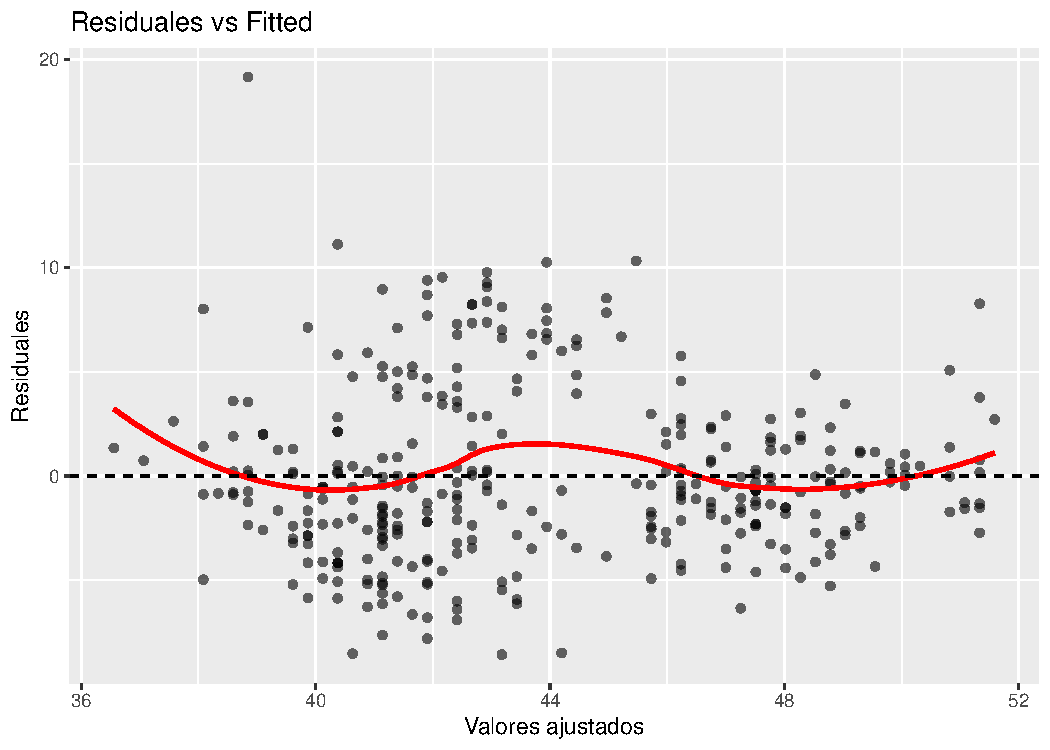
\includegraphics[keepaspectratio]{Regresiones-y-GLM_files/figure-pdf/Residuos y fitted-1.pdf}}

}

\caption{Gráfico de dispersión entre los residuales y los valores
ajustados.}

\end{figure}%

La \textbf{Figura 2} muestra que los residuos se distribuyen en torno a
la línea horizontal de cero, aunque se observa cierta curvatura y
dispersión desigual en algunos tramos. Esto indica que la relación entre
las variables no es perfectamente lineal y que podría existir cierta
heterocedasticidad (varianza no constante de los errores). Sin embargo,
no se aprecian patrones extremos que invaliden el modelo de forma
inmediata.

\begin{Shaded}
\begin{Highlighting}[numbers=left,,]
\CommentTok{\#QQ{-}plot (visual)}
\FunctionTok{ggplot}\NormalTok{(}\FunctionTok{tibble}\NormalTok{(}\AttributeTok{resid =}\NormalTok{ residuales), }\FunctionTok{aes}\NormalTok{(}\AttributeTok{sample =}\NormalTok{ resid)) }\SpecialCharTok{+}
  \FunctionTok{stat\_qq}\NormalTok{() }\SpecialCharTok{+} \FunctionTok{stat\_qq\_line}\NormalTok{() }\SpecialCharTok{+} \FunctionTok{labs}\NormalTok{(}\AttributeTok{title =} \StringTok{"QQ{-}plot de residuos"}\NormalTok{)}
\end{Highlighting}
\end{Shaded}

\begin{figure}[H]

{\centering \pandocbounded{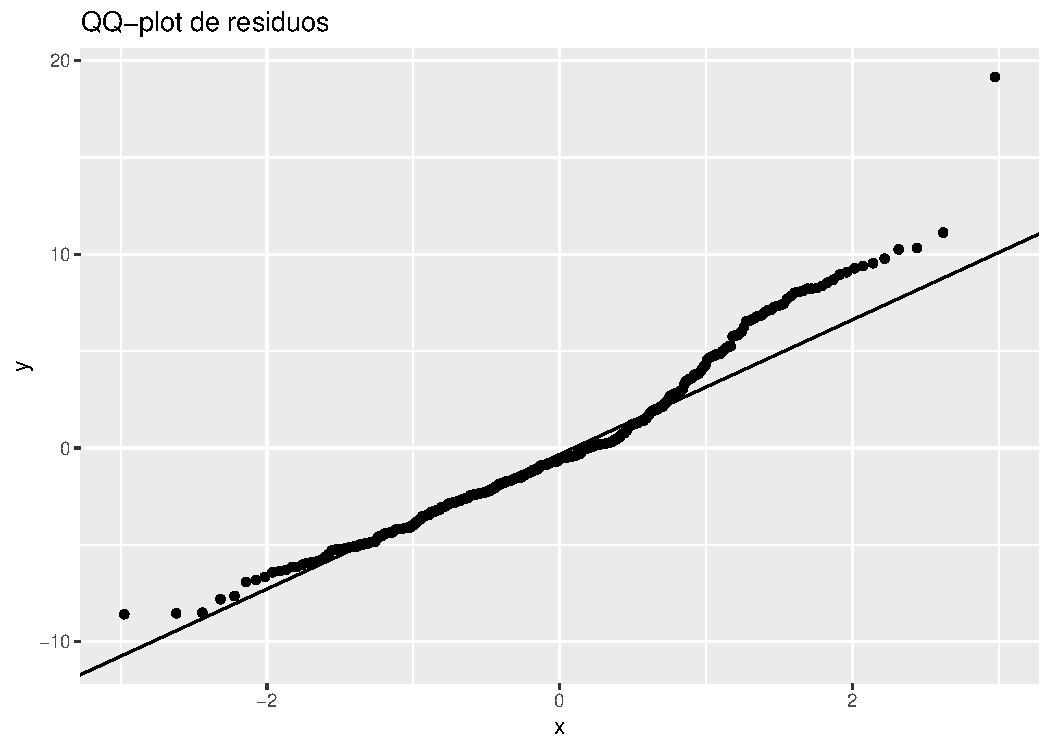
\includegraphics[keepaspectratio]{Regresiones-y-GLM_files/figure-pdf/QQ-plot-1.pdf}}

}

\caption{Gráfico QQ-plot residuos.}

\end{figure}%

La \textbf{Figura 3} refleja que la mayor parte de los puntos sigue la
línea de referencia, lo que sugiere aproximación a la normalidad. No
obstante, en las colas se observan desviaciones claras, que rechazarían
la hipótesis de normalidad. En la práctica, los modelos lineales son
relativamente robustos a esta violación cuando el tamaño de muestra es
grande, como en este caso.

\begin{Shaded}
\begin{Highlighting}[numbers=left,,]
\CommentTok{\# Tests de supuestos}

\CommentTok{\# Shapiro{-}Wilk (normalidad)}
\NormalTok{shapiro\_res }\OtherTok{\textless{}{-}}\NormalTok{ broom}\SpecialCharTok{::}\FunctionTok{tidy}\NormalTok{(}\FunctionTok{shapiro.test}\NormalTok{(residuales)) }\SpecialCharTok{\%\textgreater{}\%}
  \FunctionTok{mutate}\NormalTok{(}\AttributeTok{test =} \StringTok{"Shapiro{-}Wilk"}\NormalTok{)}

\CommentTok{\# Breusch{-}Pagan (heterocedasticidad)}
\NormalTok{bptest\_res }\OtherTok{\textless{}{-}}\NormalTok{ broom}\SpecialCharTok{::}\FunctionTok{tidy}\NormalTok{(lmtest}\SpecialCharTok{::}\FunctionTok{bptest}\NormalTok{(modelo\_lm)) }\SpecialCharTok{\%\textgreater{}\%}
  \FunctionTok{mutate}\NormalTok{(}\AttributeTok{test =} \StringTok{"Breusch{-}Pagan"}\NormalTok{)}

\CommentTok{\# Durbin{-}Watson (autocorrelación de residuos)}
\NormalTok{dw\_res }\OtherTok{\textless{}{-}}\NormalTok{ broom}\SpecialCharTok{::}\FunctionTok{tidy}\NormalTok{(lmtest}\SpecialCharTok{::}\FunctionTok{dwtest}\NormalTok{(modelo\_lm)) }\SpecialCharTok{\%\textgreater{}\%}
  \FunctionTok{mutate}\NormalTok{(}\AttributeTok{test =} \StringTok{"Durbin{-}Watson"}\NormalTok{)}

\CommentTok{\# Juntar en tabla y ajustar p{-}values}
\NormalTok{tests\_table }\OtherTok{\textless{}{-}} \FunctionTok{bind\_rows}\NormalTok{(shapiro\_res, bptest\_res, dw\_res) }\SpecialCharTok{\%\textgreater{}\%}
  \FunctionTok{select}\NormalTok{(test, statistic, p.value, method) }\SpecialCharTok{\%\textgreater{}\%}
  \FunctionTok{mutate}\NormalTok{(}
    \AttributeTok{p.value =} \FunctionTok{case\_when}\NormalTok{(}
\NormalTok{      p.value }\SpecialCharTok{\textless{}} \FloatTok{0.001} \SpecialCharTok{\textasciitilde{}} \StringTok{"\textless{} 0.001"}\NormalTok{,}
      \ConstantTok{TRUE} \SpecialCharTok{\textasciitilde{}} \FunctionTok{as.character}\NormalTok{(}\FunctionTok{round}\NormalTok{(p.value, }\DecValTok{3}\NormalTok{))}
\NormalTok{    ),}
    \AttributeTok{statistic =} \FunctionTok{round}\NormalTok{(statistic, }\DecValTok{3}\NormalTok{)}
\NormalTok{  )}

\NormalTok{knitr}\SpecialCharTok{::}\FunctionTok{kable}\NormalTok{(tests\_table, }\AttributeTok{caption =} \StringTok{"Resultados de los tests }
\StringTok{             de supuestos del modelo lineal"}\NormalTok{)}
\end{Highlighting}
\end{Shaded}

\begin{longtable}[]{@{}lrll@{}}
\caption{Resultados de los tests de supuestos del modelo
lineal}\tabularnewline
\toprule\noalign{}
test & statistic & p.value & method \\
\midrule\noalign{}
\endfirsthead
\toprule\noalign{}
test & statistic & p.value & method \\
\midrule\noalign{}
\endhead
\bottomrule\noalign{}
\endlastfoot
Shapiro-Wilk & 0.958 & \textless{} 0.001 & Shapiro-Wilk normality
test \\
Breusch-Pagan & 11.043 & \textless{} 0.001 & studentized Breusch-Pagan
test \\
Durbin-Watson & 0.939 & \textless{} 0.001 & Durbin-Watson test \\
\end{longtable}

La \textbf{Tabla 7} resume los resultados de los tests de supuestos
aplicados al modelo lineal. El test de Shapiro--Wilk indica desviaciones
de la normalidad en los residuos (p \textless{} 0.001). El test de
Breusch--Pagan es significativo (p \textless{} 0.001), lo que evidencia
heterocedasticidad, es decir, que la varianza de los errores no es
constante. Finalmente, el test de Durbin--Watson (DW = 0.939, p
\textless{} 0.001) muestra autocorrelación positiva de los residuos, lo
que sugiere dependencia entre las observaciones, posiblemente por la
estructura de especie o colonia.

\begin{Shaded}
\begin{Highlighting}[numbers=left,,]
\CommentTok{\# Calcular medidas de influencia}
\NormalTok{cooks }\OtherTok{\textless{}{-}} \FunctionTok{cooks.distance}\NormalTok{(modelo\_lm)}
\NormalTok{hatv  }\OtherTok{\textless{}{-}} \FunctionTok{hatvalues}\NormalTok{(modelo\_lm)}
\NormalTok{rstudent\_vals }\OtherTok{\textless{}{-}} \FunctionTok{rstudent}\NormalTok{(modelo\_lm)}

\CommentTok{\# Crear tabla con observaciones influyentes}
\NormalTok{influential }\OtherTok{\textless{}{-}} \FunctionTok{tibble}\NormalTok{(}
  \AttributeTok{index =} \FunctionTok{seq\_along}\NormalTok{(cooks),}
  \AttributeTok{cooks =}\NormalTok{ cooks,}
  \AttributeTok{hat =}\NormalTok{ hatv,}
  \AttributeTok{rstudent =}\NormalTok{ rstudent\_vals}
\NormalTok{) }\SpecialCharTok{\%\textgreater{}\%}
  \FunctionTok{mutate}\NormalTok{(}
    \AttributeTok{cooks\_flag =}\NormalTok{ cooks }\SpecialCharTok{\textgreater{}}\NormalTok{ (}\DecValTok{4}\SpecialCharTok{/}\FunctionTok{length}\NormalTok{(cooks)),}
    \AttributeTok{rstudent\_flag =} \FunctionTok{abs}\NormalTok{(rstudent) }\SpecialCharTok{\textgreater{}} \DecValTok{3}\NormalTok{,}
    \AttributeTok{hat\_flag =}\NormalTok{ hat }\SpecialCharTok{\textgreater{}}\NormalTok{ (}\DecValTok{2}\SpecialCharTok{*}\NormalTok{(k}\SpecialCharTok{+}\DecValTok{1}\NormalTok{)}\SpecialCharTok{/}\NormalTok{n)}
\NormalTok{  ) }\SpecialCharTok{\%\textgreater{}\%}
  \FunctionTok{filter}\NormalTok{(cooks\_flag }\SpecialCharTok{|}\NormalTok{ rstudent\_flag }\SpecialCharTok{|}\NormalTok{ hat\_flag) }\SpecialCharTok{\%\textgreater{}\%}
  \FunctionTok{arrange}\NormalTok{(}\FunctionTok{desc}\NormalTok{(cooks)) }\SpecialCharTok{\%\textgreater{}\%}
  \FunctionTok{mutate}\NormalTok{(}\FunctionTok{across}\NormalTok{(}\FunctionTok{where}\NormalTok{(is.numeric), round, }\DecValTok{3}\NormalTok{))}

\NormalTok{knitr}\SpecialCharTok{::}\FunctionTok{kable}\NormalTok{(influential, }\AttributeTok{caption =} \StringTok{"Observaciones potencialmente }
\StringTok{             influyentes (Cook’s distance, leverage, residuos studentizados)"}\NormalTok{)}
\end{Highlighting}
\end{Shaded}

\begin{longtable}[]{@{}rrrrlll@{}}
\caption{Observaciones potencialmente influyentes (Cook's distance,
leverage, residuos studentizados)}\tabularnewline
\toprule\noalign{}
index & cooks & hat & rstudent & cooks\_flag & rstudent\_flag &
hat\_flag \\
\midrule\noalign{}
\endfirsthead
\toprule\noalign{}
index & cooks & hat & rstudent & cooks\_flag & rstudent\_flag &
hat\_flag \\
\midrule\noalign{}
\endhead
\bottomrule\noalign{}
\endlastfoot
292 & 0.097 & 0.009 & 4.812 & TRUE & TRUE & FALSE \\
185 & 0.032 & 0.015 & 2.029 & TRUE & FALSE & TRUE \\
323 & 0.021 & 0.006 & 2.729 & TRUE & FALSE & FALSE \\
281 & 0.021 & 0.011 & 1.962 & TRUE & FALSE & FALSE \\
253 & 0.011 & 0.014 & 1.240 & FALSE & FALSE & TRUE \\
267 & 0.007 & 0.015 & 0.920 & FALSE & FALSE & TRUE \\
215 & 0.004 & 0.016 & 0.663 & FALSE & FALSE & TRUE \\
227 & 0.003 & 0.015 & -0.667 & FALSE & FALSE & TRUE \\
122 & 0.003 & 0.012 & 0.640 & FALSE & FALSE & TRUE \\
255 & 0.001 & 0.014 & -0.420 & FALSE & FALSE & TRUE \\
219 & 0.001 & 0.015 & -0.385 & FALSE & FALSE & TRUE \\
217 & 0.001 & 0.015 & -0.374 & FALSE & FALSE & TRUE \\
28 & 0.001 & 0.015 & 0.328 & FALSE & FALSE & TRUE \\
153 & 0.001 & 0.015 & -0.325 & FALSE & FALSE & TRUE \\
243 & 0.001 & 0.014 & 0.336 & FALSE & FALSE & TRUE \\
263 & 0.001 & 0.015 & -0.311 & FALSE & FALSE & TRUE \\
241 & 0.000 & 0.015 & 0.187 & FALSE & FALSE & TRUE \\
20 & 0.000 & 0.014 & 0.179 & FALSE & FALSE & TRUE \\
247 & 0.000 & 0.012 & 0.119 & FALSE & FALSE & TRUE \\
265 & 0.000 & 0.015 & 0.041 & FALSE & FALSE & TRUE \\
237 & 0.000 & 0.014 & -0.005 & FALSE & FALSE & TRUE \\
\end{longtable}

La \textbf{Tabla 8} presenta las observaciones potencialmente
influyentes detectadas mediante Cook's distance, leverage y residuos
studentizados. Destaca la observación 292, con un residuo estudentizado
muy alto (4.81) y una distancia de Cook por encima del umbral (0.097),
lo que indica que afecta fuertemente los parámetros estimados. Las
observaciones 185 y 323 también muestran valores de Cook elevados y, en
el caso de 185, un leverage alto, lo que refleja un peso excesivo en el
ajuste. El resto de observaciones (e.g., 281, 253, 267) presentan
leverage relativamente alto, pero con menor impacto individual en el
modelo.

Desde una perspectiva biológica, estas observaciones pueden corresponder
a individuos atípicos, errores de medición o variabilidad natural de las
poblaciones, y su tratamiento debe basarse en criterios ecológicos
además de estadísticos.

\begin{Shaded}
\begin{Highlighting}[numbers=left,,]
\CommentTok{\# Crear modelo sin observaciones influyentes y comparar coeficientes}
\NormalTok{in\_idx }\OtherTok{\textless{}{-}}\NormalTok{ influential}\SpecialCharTok{$}\NormalTok{index}

\ControlFlowTok{if}\NormalTok{(}\FunctionTok{length}\NormalTok{(in\_idx) }\SpecialCharTok{\textgreater{}} \DecValTok{0}\NormalTok{)\{}
\NormalTok{  modelo\_lm\_noinf }\OtherTok{\textless{}{-}} \FunctionTok{lm}\NormalTok{(bill\_length\_mm }\SpecialCharTok{\textasciitilde{}}\NormalTok{ flipper\_length\_mm,}
                        \AttributeTok{data =}\NormalTok{ df[}\SpecialCharTok{{-}}\NormalTok{in\_idx, ])}
  
\NormalTok{  compare\_coefs }\OtherTok{\textless{}{-}} \FunctionTok{tibble}\NormalTok{(}
    \AttributeTok{original =}\NormalTok{ broom}\SpecialCharTok{::}\FunctionTok{tidy}\NormalTok{(modelo\_lm)}\SpecialCharTok{$}\NormalTok{estimate,}
    \AttributeTok{no\_influ =}\NormalTok{ broom}\SpecialCharTok{::}\FunctionTok{tidy}\NormalTok{(modelo\_lm\_noinf)}\SpecialCharTok{$}\NormalTok{estimate}
\NormalTok{  )}
  
\NormalTok{  knitr}\SpecialCharTok{::}\FunctionTok{kable}\NormalTok{(}
\NormalTok{    compare\_coefs }\SpecialCharTok{\%\textgreater{}\%}
      \FunctionTok{mutate}\NormalTok{(}\FunctionTok{across}\NormalTok{(}\FunctionTok{where}\NormalTok{(is.numeric), round, }\DecValTok{3}\NormalTok{)) }\SpecialCharTok{\%\textgreater{}\%}
      \FunctionTok{rename}\NormalTok{(}\StringTok{"Modelo original"} \OtherTok{=}\NormalTok{ original,}
             \StringTok{"Modelo sin influyentes"} \OtherTok{=}\NormalTok{ no\_influ),}
    \AttributeTok{caption =} \StringTok{"Comparación de coeficientes estimados con }
\StringTok{    y sin observaciones influyentes."}
\NormalTok{  )}
\NormalTok{\} }\ControlFlowTok{else}\NormalTok{ \{}
  \StringTok{"No se detectaron observaciones influyentes con los umbrales establecidos."}
\NormalTok{\}}
\end{Highlighting}
\end{Shaded}

\begin{longtable}[]{@{}rr@{}}
\caption{Comparación de coeficientes estimados con y sin observaciones
influyentes.}\tabularnewline
\toprule\noalign{}
Modelo original & Modelo sin influyentes \\
\midrule\noalign{}
\endfirsthead
\toprule\noalign{}
Modelo original & Modelo sin influyentes \\
\midrule\noalign{}
\endhead
\bottomrule\noalign{}
\endlastfoot
-7.265 & -9.128 \\
0.255 & 0.263 \\
\end{longtable}

La \textbf{Tabla 9} muestra los coeficientes estimados para el modelo
original y para el modelo ajustado sin las observaciones influyentes (n
= 21). Se observa que el intercepto cambia de --7.26 a --9.13, y la
pendiente de 0.255 a 0.263. Aunque los cambios son moderados, evidencian
que las observaciones influyentes, especialmente la 292, tienen un
impacto en la magnitud de los parámetros.

\section{Conclusiones del modelo
lineal}\label{conclusiones-del-modelo-lineal}

El modelo lineal confirma una relación positiva fuerte entre el largo
del ala y el largo del pico en pingüinos, aunque presenta violaciones a
varios supuestos:

\begin{itemize}
\item
  Normalidad: los residuos no siguen una distribución normal
  (Shapiro-Wilk significativo).
\item
  Homoscedasticidad: la varianza de los errores no es constante
  (Breusch-Pagan significativo).
\item
  Independencia: los residuos presentan autocorrelación positiva
  (Durbin-Watson).
\item
  Influencia de outliers: algunas observaciones (p.~ej., la 292) afectan
  de manera importante el ajuste.
\end{itemize}

Estos resultados sugieren que, si bien el modelo lineal simple ofrece
información valiosa, es necesario avanzar hacia enfoques más robustos:

\begin{itemize}
\item
  Evaluar modelos que incluyan variables adicionales (como especie o
  sexo).
\item
  Considerar modelos lineales generalizados o mixtos que controlen por
  estructura de datos y agrupamiento.
\item
  Explorar la posibilidad de transformaciones o métodos robustos frente
  a outliers.
\item
  En síntesis, la relación biológica entre largo de ala y pico es clara
  y significativa, pero el modelo lineal simple debe interpretarse con
  cautela debido a las violaciones de supuestos y la influencia de casos
  extremos.
\end{itemize}

\section{Regresión lineal
múltiple}\label{regresiuxf3n-lineal-muxfaltiple}

En vez de usar solo \texttt{flipper\_length\_mm} como predictor del
\texttt{bill\_length\_mm}, ahora incluiremos la especie como variable
categórica. Esto nos permite responder:

\begin{itemize}
\item
  ¿Sigue siendo significativa la relación entre longitud de ala y pico,
  una vez controlamos por especie?
\item
  ¿Existen diferencias en la longitud del pico atribuibles directamente
  a la especie?
\end{itemize}

\begin{Shaded}
\begin{Highlighting}[numbers=left,,]
\CommentTok{\# Modelo de regresión múltiple: bill\_length \textasciitilde{} flipper\_length + species}
\NormalTok{modelo\_lm\_multi }\OtherTok{\textless{}{-}} \FunctionTok{lm}\NormalTok{(bill\_length\_mm }\SpecialCharTok{\textasciitilde{}}\NormalTok{ flipper\_length\_mm }\SpecialCharTok{+}\NormalTok{ species, }\AttributeTok{data =}\NormalTok{ df)}

\CommentTok{\# Resumen de coeficientes}
\NormalTok{tabla\_multi }\OtherTok{\textless{}{-}}\NormalTok{ broom}\SpecialCharTok{::}\FunctionTok{tidy}\NormalTok{(modelo\_lm\_multi, }\AttributeTok{conf.int =} \ConstantTok{TRUE}\NormalTok{)}

\NormalTok{knitr}\SpecialCharTok{::}\FunctionTok{kable}\NormalTok{(}
\NormalTok{  tabla\_multi }\SpecialCharTok{\%\textgreater{}\%}
    \FunctionTok{mutate}\NormalTok{(}\FunctionTok{across}\NormalTok{(}\FunctionTok{where}\NormalTok{(is.numeric), round, }\DecValTok{3}\NormalTok{)),}
  \AttributeTok{caption =} \StringTok{"Coeficientes estimados del modelo lineal múltiple }
\StringTok{  (longitud del pico como variable respuesta)."}
\NormalTok{)}
\end{Highlighting}
\end{Shaded}

\begin{longtable}[]{@{}
  >{\raggedright\arraybackslash}p{(\linewidth - 12\tabcolsep) * \real{0.2432}}
  >{\raggedleft\arraybackslash}p{(\linewidth - 12\tabcolsep) * \real{0.1216}}
  >{\raggedleft\arraybackslash}p{(\linewidth - 12\tabcolsep) * \real{0.1351}}
  >{\raggedleft\arraybackslash}p{(\linewidth - 12\tabcolsep) * \real{0.1351}}
  >{\raggedleft\arraybackslash}p{(\linewidth - 12\tabcolsep) * \real{0.1081}}
  >{\raggedleft\arraybackslash}p{(\linewidth - 12\tabcolsep) * \real{0.1216}}
  >{\raggedleft\arraybackslash}p{(\linewidth - 12\tabcolsep) * \real{0.1351}}@{}}
\caption{Coeficientes estimados del modelo lineal múltiple (longitud del
pico como variable respuesta).}\tabularnewline
\toprule\noalign{}
\begin{minipage}[b]{\linewidth}\raggedright
term
\end{minipage} & \begin{minipage}[b]{\linewidth}\raggedleft
estimate
\end{minipage} & \begin{minipage}[b]{\linewidth}\raggedleft
std.error
\end{minipage} & \begin{minipage}[b]{\linewidth}\raggedleft
statistic
\end{minipage} & \begin{minipage}[b]{\linewidth}\raggedleft
p.value
\end{minipage} & \begin{minipage}[b]{\linewidth}\raggedleft
conf.low
\end{minipage} & \begin{minipage}[b]{\linewidth}\raggedleft
conf.high
\end{minipage} \\
\midrule\noalign{}
\endfirsthead
\toprule\noalign{}
\begin{minipage}[b]{\linewidth}\raggedright
term
\end{minipage} & \begin{minipage}[b]{\linewidth}\raggedleft
estimate
\end{minipage} & \begin{minipage}[b]{\linewidth}\raggedleft
std.error
\end{minipage} & \begin{minipage}[b]{\linewidth}\raggedleft
statistic
\end{minipage} & \begin{minipage}[b]{\linewidth}\raggedleft
p.value
\end{minipage} & \begin{minipage}[b]{\linewidth}\raggedleft
conf.low
\end{minipage} & \begin{minipage}[b]{\linewidth}\raggedleft
conf.high
\end{minipage} \\
\midrule\noalign{}
\endhead
\bottomrule\noalign{}
\endlastfoot
(Intercept) & -2.059 & 4.039 & -0.510 & 0.611 & -10.002 & 5.885 \\
flipper\_length\_mm & 0.215 & 0.021 & 10.129 & 0.000 & 0.173 & 0.257 \\
speciesChinstrap & 8.780 & 0.399 & 21.998 & 0.000 & 7.995 & 9.565 \\
speciesGentoo & 2.857 & 0.659 & 4.338 & 0.000 & 1.561 & 4.152 \\
\end{longtable}

La \textbf{Tabla 10} muestra los coeficientes del modelo múltiple que
relaciona la longitud del pico (\texttt{bill\_length\_mm}) con la
longitud del ala (\texttt{flipper\_length\_mm}) y la especie.

\begin{itemize}
\item
  El intercepto (β0 = -2.06, p = 0.611) no es significativo y representa
  la longitud promedio del pico para pingüinos \emph{Adelie} (categoría
  de referencia) con longitud de ala igual a cero. Este valor carece de
  interpretación biológica directa, pero es necesario para el modelo.
\item
  El coeficiente de \texttt{flipper\_length\_mm} (β1 = 0.215, p
  \textless{} 0.001) indica que, controlando por especie, un aumento de
  1 mm en la longitud del ala se asocia con un incremento promedio de
  0.215 mm en la longitud del pico. Esto confirma una relación
  alométrica positiva entre el tamaño corporal y la morfología del pico
  dentro de cada especie.
\item
  La especie \emph{Chinstrap} presenta un pico en promedio 8.78 mm más
  largo que los \emph{Adelie} (p \textless{} 0.001), mientras que los
  \emph{Gentoo} presentan picos 2.86 mm más largos que los \emph{Adelie}
  (p \textless{} 0.001), ajustando por longitud del ala. Estas
  diferencias son significativas y reflejan divergencias morfológicas
  marcadas entre especies.
\end{itemize}

\begin{Shaded}
\begin{Highlighting}[numbers=left,,]
\CommentTok{\# Métricas generales del modelo}
\NormalTok{tabla\_multi\_glance }\OtherTok{\textless{}{-}}\NormalTok{ broom}\SpecialCharTok{::}\FunctionTok{glance}\NormalTok{(modelo\_lm\_multi)}

\NormalTok{knitr}\SpecialCharTok{::}\FunctionTok{kable}\NormalTok{(}
\NormalTok{  tabla\_multi\_glance }\SpecialCharTok{\%\textgreater{}\%}
    \FunctionTok{mutate}\NormalTok{(}\FunctionTok{across}\NormalTok{(}\FunctionTok{where}\NormalTok{(is.numeric), round, }\DecValTok{3}\NormalTok{)),}
  \AttributeTok{caption =} \StringTok{"Estadísticos de ajuste del modelo múltiple."}
\NormalTok{)}
\end{Highlighting}
\end{Shaded}

\begin{longtable}[]{@{}
  >{\raggedleft\arraybackslash}p{(\linewidth - 22\tabcolsep) * \real{0.0971}}
  >{\raggedleft\arraybackslash}p{(\linewidth - 22\tabcolsep) * \real{0.1359}}
  >{\raggedleft\arraybackslash}p{(\linewidth - 22\tabcolsep) * \real{0.0583}}
  >{\raggedleft\arraybackslash}p{(\linewidth - 22\tabcolsep) * \real{0.0971}}
  >{\raggedleft\arraybackslash}p{(\linewidth - 22\tabcolsep) * \real{0.0777}}
  >{\raggedleft\arraybackslash}p{(\linewidth - 22\tabcolsep) * \real{0.0291}}
  >{\raggedleft\arraybackslash}p{(\linewidth - 22\tabcolsep) * \real{0.0777}}
  >{\raggedleft\arraybackslash}p{(\linewidth - 22\tabcolsep) * \real{0.0874}}
  >{\raggedleft\arraybackslash}p{(\linewidth - 22\tabcolsep) * \real{0.0874}}
  >{\raggedleft\arraybackslash}p{(\linewidth - 22\tabcolsep) * \real{0.0874}}
  >{\raggedleft\arraybackslash}p{(\linewidth - 22\tabcolsep) * \real{0.1165}}
  >{\raggedleft\arraybackslash}p{(\linewidth - 22\tabcolsep) * \real{0.0485}}@{}}
\caption{Estadísticos de ajuste del modelo múltiple.}\tabularnewline
\toprule\noalign{}
\begin{minipage}[b]{\linewidth}\raggedleft
r.squared
\end{minipage} & \begin{minipage}[b]{\linewidth}\raggedleft
adj.r.squared
\end{minipage} & \begin{minipage}[b]{\linewidth}\raggedleft
sigma
\end{minipage} & \begin{minipage}[b]{\linewidth}\raggedleft
statistic
\end{minipage} & \begin{minipage}[b]{\linewidth}\raggedleft
p.value
\end{minipage} & \begin{minipage}[b]{\linewidth}\raggedleft
df
\end{minipage} & \begin{minipage}[b]{\linewidth}\raggedleft
logLik
\end{minipage} & \begin{minipage}[b]{\linewidth}\raggedleft
AIC
\end{minipage} & \begin{minipage}[b]{\linewidth}\raggedleft
BIC
\end{minipage} & \begin{minipage}[b]{\linewidth}\raggedleft
deviance
\end{minipage} & \begin{minipage}[b]{\linewidth}\raggedleft
df.residual
\end{minipage} & \begin{minipage}[b]{\linewidth}\raggedleft
nobs
\end{minipage} \\
\midrule\noalign{}
\endfirsthead
\toprule\noalign{}
\begin{minipage}[b]{\linewidth}\raggedleft
r.squared
\end{minipage} & \begin{minipage}[b]{\linewidth}\raggedleft
adj.r.squared
\end{minipage} & \begin{minipage}[b]{\linewidth}\raggedleft
sigma
\end{minipage} & \begin{minipage}[b]{\linewidth}\raggedleft
statistic
\end{minipage} & \begin{minipage}[b]{\linewidth}\raggedleft
p.value
\end{minipage} & \begin{minipage}[b]{\linewidth}\raggedleft
df
\end{minipage} & \begin{minipage}[b]{\linewidth}\raggedleft
logLik
\end{minipage} & \begin{minipage}[b]{\linewidth}\raggedleft
AIC
\end{minipage} & \begin{minipage}[b]{\linewidth}\raggedleft
BIC
\end{minipage} & \begin{minipage}[b]{\linewidth}\raggedleft
deviance
\end{minipage} & \begin{minipage}[b]{\linewidth}\raggedleft
df.residual
\end{minipage} & \begin{minipage}[b]{\linewidth}\raggedleft
nobs
\end{minipage} \\
\midrule\noalign{}
\endhead
\bottomrule\noalign{}
\endlastfoot
0.776 & 0.774 & 2.596 & 389.966 & 0 & 3 & -809.56 & 1629.119 & 1648.294
& 2278.337 & 338 & 342 \\
\end{longtable}

La \textbf{Tabla 11} muestra los estadísticos globales del ajuste. El
modelo explica un 77.6\% de la variabilidad en la longitud del pico (R²
= 0.776), lo cual representa una mejora sustancial respecto al modelo
simple (R² ≈ 0.43). El error residual (σ = 2.60 mm) es considerablemente
menor que en el modelo simple, indicando un mejor ajuste.

En conjunto, el modelo múltiple sugiere que tanto el tamaño corporal
(longitud de ala) como la especie son predictores clave de la longitud
del pico. Desde un punto de vista ecológico, esto refleja que la
morfología del pico no solo está asociada al tamaño general del cuerpo,
sino que también depende de adaptaciones específicas entre especies,
posiblemente vinculadas a diferencias en dieta, ecología trófica o
hábitat.

\begin{Shaded}
\begin{Highlighting}[numbers=left,,]
\CommentTok{\# Comparar modelo simple vs múltiple}
\NormalTok{modelo\_simple }\OtherTok{\textless{}{-}} \FunctionTok{lm}\NormalTok{(bill\_length\_mm }\SpecialCharTok{\textasciitilde{}}\NormalTok{ flipper\_length\_mm, }\AttributeTok{data =}\NormalTok{ df)}
\NormalTok{modelo\_multiple }\OtherTok{\textless{}{-}} \FunctionTok{lm}\NormalTok{(bill\_length\_mm }\SpecialCharTok{\textasciitilde{}}\NormalTok{ flipper\_length\_mm }\SpecialCharTok{+}\NormalTok{ species, }\AttributeTok{data =}\NormalTok{ df)}

\CommentTok{\# Extraer métricas de ajuste}
\NormalTok{comp\_models }\OtherTok{\textless{}{-}} \FunctionTok{bind\_rows}\NormalTok{(}
\NormalTok{  broom}\SpecialCharTok{::}\FunctionTok{glance}\NormalTok{(modelo\_simple) }\SpecialCharTok{\%\textgreater{}\%} \FunctionTok{mutate}\NormalTok{(}\AttributeTok{modelo =} \StringTok{"Simple"}\NormalTok{),}
\NormalTok{  broom}\SpecialCharTok{::}\FunctionTok{glance}\NormalTok{(modelo\_multiple) }\SpecialCharTok{\%\textgreater{}\%} \FunctionTok{mutate}\NormalTok{(}\AttributeTok{modelo =} \StringTok{"Múltiple"}\NormalTok{)}
\NormalTok{) }\SpecialCharTok{\%\textgreater{}\%}
  \FunctionTok{select}\NormalTok{(modelo, r.squared, adj.r.squared, AIC, BIC, sigma, p.value) }\SpecialCharTok{\%\textgreater{}\%}
  \FunctionTok{mutate}\NormalTok{(}\FunctionTok{across}\NormalTok{(}\FunctionTok{where}\NormalTok{(is.numeric), }\SpecialCharTok{\textasciitilde{}}\FunctionTok{round}\NormalTok{(., }\DecValTok{3}\NormalTok{)))}

\NormalTok{knitr}\SpecialCharTok{::}\FunctionTok{kable}\NormalTok{(comp\_models,}
             \AttributeTok{caption =} \StringTok{"Comparación entre el modelo }
\StringTok{             lineal simple y múltiple"}\NormalTok{)}
\end{Highlighting}
\end{Shaded}

\begin{longtable}[]{@{}
  >{\raggedright\arraybackslash}p{(\linewidth - 12\tabcolsep) * \real{0.1385}}
  >{\raggedleft\arraybackslash}p{(\linewidth - 12\tabcolsep) * \real{0.1538}}
  >{\raggedleft\arraybackslash}p{(\linewidth - 12\tabcolsep) * \real{0.2154}}
  >{\raggedleft\arraybackslash}p{(\linewidth - 12\tabcolsep) * \real{0.1385}}
  >{\raggedleft\arraybackslash}p{(\linewidth - 12\tabcolsep) * \real{0.1385}}
  >{\raggedleft\arraybackslash}p{(\linewidth - 12\tabcolsep) * \real{0.0923}}
  >{\raggedleft\arraybackslash}p{(\linewidth - 12\tabcolsep) * \real{0.1231}}@{}}
\caption{Comparación entre el modelo lineal simple y
múltiple}\tabularnewline
\toprule\noalign{}
\begin{minipage}[b]{\linewidth}\raggedright
modelo
\end{minipage} & \begin{minipage}[b]{\linewidth}\raggedleft
r.squared
\end{minipage} & \begin{minipage}[b]{\linewidth}\raggedleft
adj.r.squared
\end{minipage} & \begin{minipage}[b]{\linewidth}\raggedleft
AIC
\end{minipage} & \begin{minipage}[b]{\linewidth}\raggedleft
BIC
\end{minipage} & \begin{minipage}[b]{\linewidth}\raggedleft
sigma
\end{minipage} & \begin{minipage}[b]{\linewidth}\raggedleft
p.value
\end{minipage} \\
\midrule\noalign{}
\endfirsthead
\toprule\noalign{}
\begin{minipage}[b]{\linewidth}\raggedright
modelo
\end{minipage} & \begin{minipage}[b]{\linewidth}\raggedleft
r.squared
\end{minipage} & \begin{minipage}[b]{\linewidth}\raggedleft
adj.r.squared
\end{minipage} & \begin{minipage}[b]{\linewidth}\raggedleft
AIC
\end{minipage} & \begin{minipage}[b]{\linewidth}\raggedleft
BIC
\end{minipage} & \begin{minipage}[b]{\linewidth}\raggedleft
sigma
\end{minipage} & \begin{minipage}[b]{\linewidth}\raggedleft
p.value
\end{minipage} \\
\midrule\noalign{}
\endhead
\bottomrule\noalign{}
\endlastfoot
Simple & 0.431 & 0.429 & 1943.966 & 1955.471 & 4.126 & 0 \\
Múltiple & 0.776 & 0.774 & 1629.119 & 1648.294 & 2.596 & 0 \\
\end{longtable}

La \textbf{Tabla 12} compara el modelo lineal simple y el múltiple. El
modelo simple (solo con la longitud del ala) explica alrededor del 43\%
de la variación en la longitud del pico (R² = 0.431), mientras que el
modelo múltiple (incluyendo la especie) aumenta notablemente la
capacidad explicativa hasta un 77\% (R² = 0.776).

Además, los criterios de información (AIC y BIC) son considerablemente
menores en el modelo múltiple, lo que indica un mejor ajuste penalizado
por complejidad. En conjunto, la comparación sugiere que la variable
especie aporta información fundamental para explicar las diferencias en
la longitud del pico, más allá del tamaño corporal.

\section{Diagnósticos del modelo
múltiple}\label{diagnuxf3sticos-del-modelo-muxfaltiple}

\begin{Shaded}
\begin{Highlighting}[numbers=left,,]
\CommentTok{\# Residuos del modelo múltiple}
\NormalTok{residuales\_m }\OtherTok{\textless{}{-}} \FunctionTok{resid}\NormalTok{(modelo\_multiple)}

\CommentTok{\# Pruebas de supuestos}
\NormalTok{shapiro\_res\_m }\OtherTok{\textless{}{-}} \FunctionTok{shapiro.test}\NormalTok{(residuales\_m)}
\NormalTok{bptest\_res\_m  }\OtherTok{\textless{}{-}}\NormalTok{ lmtest}\SpecialCharTok{::}\FunctionTok{bptest}\NormalTok{(modelo\_multiple)}
\NormalTok{dw\_res\_m      }\OtherTok{\textless{}{-}}\NormalTok{ lmtest}\SpecialCharTok{::}\FunctionTok{dwtest}\NormalTok{(modelo\_multiple)}

\CommentTok{\# Resumen en tabla}
\NormalTok{tests\_table\_m }\OtherTok{\textless{}{-}} \FunctionTok{tibble}\NormalTok{(}
  \AttributeTok{Test =} \FunctionTok{c}\NormalTok{(}\StringTok{"Shapiro{-}Wilk (normalidad)"}\NormalTok{,}
           \StringTok{"Breusch{-}Pagan (homocedasticidad)"}\NormalTok{,}
           \StringTok{"Durbin{-}Watson (independencia)"}\NormalTok{),}
\NormalTok{  Estadístico }\OtherTok{=} \FunctionTok{c}\NormalTok{(}\FunctionTok{round}\NormalTok{(shapiro\_res\_m}\SpecialCharTok{$}\NormalTok{statistic, }\DecValTok{3}\NormalTok{),}
                  \FunctionTok{round}\NormalTok{(bptest\_res\_m}\SpecialCharTok{$}\NormalTok{statistic, }\DecValTok{3}\NormalTok{),}
                  \FunctionTok{round}\NormalTok{(dw\_res\_m}\SpecialCharTok{$}\NormalTok{statistic, }\DecValTok{3}\NormalTok{)),}
  \AttributeTok{p\_value =} \FunctionTok{c}\NormalTok{(}\FunctionTok{ifelse}\NormalTok{(shapiro\_res\_m}\SpecialCharTok{$}\NormalTok{p.value }\SpecialCharTok{\textless{}} \FloatTok{0.001}\NormalTok{, }\StringTok{"\textless{}0.001"}\NormalTok{, }
                     \FunctionTok{round}\NormalTok{(shapiro\_res\_m}\SpecialCharTok{$}\NormalTok{p.value, }\DecValTok{3}\NormalTok{)),}
              \FunctionTok{ifelse}\NormalTok{(bptest\_res\_m}\SpecialCharTok{$}\NormalTok{p.value }\SpecialCharTok{\textless{}} \FloatTok{0.001}\NormalTok{, }\StringTok{"\textless{}0.001"}\NormalTok{, }
                     \FunctionTok{round}\NormalTok{(bptest\_res\_m}\SpecialCharTok{$}\NormalTok{p.value, }\DecValTok{3}\NormalTok{)),}
              \FunctionTok{ifelse}\NormalTok{(dw\_res\_m}\SpecialCharTok{$}\NormalTok{p.value }\SpecialCharTok{\textless{}} \FloatTok{0.001}\NormalTok{, }\StringTok{"\textless{}0.001"}\NormalTok{, }
                     \FunctionTok{round}\NormalTok{(dw\_res\_m}\SpecialCharTok{$}\NormalTok{p.value, }\DecValTok{3}\NormalTok{)))}
\NormalTok{)}

\NormalTok{knitr}\SpecialCharTok{::}\FunctionTok{kable}\NormalTok{(tests\_table\_m,}
             \AttributeTok{caption =} \StringTok{"Resultados de las pruebas de }
\StringTok{             supuestos del modelo múltiple"}\NormalTok{)}
\end{Highlighting}
\end{Shaded}

\begin{longtable}[]{@{}lrr@{}}
\caption{Resultados de las pruebas de supuestos del modelo
múltiple}\tabularnewline
\toprule\noalign{}
Test & Estadístico & p\_value \\
\midrule\noalign{}
\endfirsthead
\toprule\noalign{}
Test & Estadístico & p\_value \\
\midrule\noalign{}
\endhead
\bottomrule\noalign{}
\endlastfoot
Shapiro-Wilk (normalidad) & 0.985 & 0.001 \\
Breusch-Pagan (homocedasticidad) & 2.923 & 0.404 \\
Durbin-Watson (independencia) & 2.450 & 1.000 \\
\end{longtable}

La \textbf{Tabla 13} presenta las pruebas de supuestos del modelo lineal
múltiple. El test de Shapiro-Wilk indica un valor \emph{p = 0.001}, lo
que sugiere que los residuos se desvían de una distribución normal
perfecta. Sin embargo, dado el tamaño de la muestra, pequeñas
desviaciones pueden detectarse como significativas sin afectar
sustancialmente la validez del modelo. El test de Breusch-Pagan (\emph{p
= 0.404}) no rechaza la hipótesis de homocedasticidad, por lo que no hay
evidencia de heterocedasticidad. Por su parte, el test de Durbin-Watson
muestra un valor cercano a 2 (\emph{p = 1.000}), lo que respalda la
ausencia de autocorrelación en los residuos. En conjunto, estos
resultados sugieren que los supuestos principales de homogeneidad e
independencia se cumplen, mientras que la normalidad de los residuos
presenta una ligera desviación.

\begin{Shaded}
\begin{Highlighting}[numbers=left,,]
\CommentTok{\# Influencia en el modelo múltiple}
\NormalTok{cooks\_m }\OtherTok{\textless{}{-}} \FunctionTok{cooks.distance}\NormalTok{(modelo\_multiple)}
\NormalTok{hatv\_m  }\OtherTok{\textless{}{-}} \FunctionTok{hatvalues}\NormalTok{(modelo\_multiple)}
\NormalTok{rstud\_m }\OtherTok{\textless{}{-}} \FunctionTok{rstudent}\NormalTok{(modelo\_multiple)}

\NormalTok{influential\_m }\OtherTok{\textless{}{-}} \FunctionTok{tibble}\NormalTok{(}
  \AttributeTok{index =} \FunctionTok{seq\_along}\NormalTok{(cooks\_m),}
  \AttributeTok{cooks =}\NormalTok{ cooks\_m,}
  \AttributeTok{leverage =}\NormalTok{ hatv\_m,}
  \AttributeTok{rstudent =}\NormalTok{ rstud\_m}
\NormalTok{) }\SpecialCharTok{\%\textgreater{}\%}
  \FunctionTok{filter}\NormalTok{(cooks }\SpecialCharTok{\textgreater{}} \DecValTok{4}\SpecialCharTok{/}\FunctionTok{length}\NormalTok{(cooks\_m) }\SpecialCharTok{|} \FunctionTok{abs}\NormalTok{(rstudent) }\SpecialCharTok{\textgreater{}} \DecValTok{3}\NormalTok{) }\SpecialCharTok{\%\textgreater{}\%}
  \FunctionTok{mutate}\NormalTok{(}\FunctionTok{across}\NormalTok{(}\FunctionTok{where}\NormalTok{(is.numeric), round, }\DecValTok{3}\NormalTok{))}

\NormalTok{knitr}\SpecialCharTok{::}\FunctionTok{kable}\NormalTok{(influential\_m,}
             \AttributeTok{caption =} \StringTok{"Observaciones potencialmente }
\StringTok{             influyentes en el modelo múltiple"}\NormalTok{)}
\end{Highlighting}
\end{Shaded}

\begin{longtable}[]{@{}rrrr@{}}
\caption{Observaciones potencialmente influyentes en el modelo
múltiple}\tabularnewline
\toprule\noalign{}
index & cooks & leverage & rstudent \\
\midrule\noalign{}
\endfirsthead
\toprule\noalign{}
index & cooks & leverage & rstudent \\
\midrule\noalign{}
\endhead
\bottomrule\noalign{}
\endlastfoot
14 & 0.015 & 0.011 & -2.308 \\
37 & 0.016 & 0.013 & 2.163 \\
90 & 0.020 & 0.016 & -2.219 \\
122 & 0.015 & 0.020 & 1.720 \\
185 & 0.064 & 0.019 & 3.700 \\
215 & 0.012 & 0.021 & 1.491 \\
250 & 0.013 & 0.022 & 1.540 \\
253 & 0.023 & 0.016 & 2.373 \\
267 & 0.017 & 0.019 & 1.889 \\
292 & 0.177 & 0.029 & 4.998 \\
295 & 0.012 & 0.029 & -1.270 \\
305 & 0.028 & 0.020 & -2.364 \\
307 & 0.015 & 0.020 & -1.731 \\
322 & 0.014 & 0.032 & -1.298 \\
323 & 0.016 & 0.020 & 1.781 \\
329 & 0.015 & 0.020 & -1.731 \\
338 & 0.019 & 0.023 & 1.784 \\
339 & 0.029 & 0.017 & -2.611 \\
\end{longtable}

La \textbf{Tabla 14} muestra las observaciones potencialmente
influyentes según Cook's distance, leverage y residuos studentizados. En
particular, los casos 185 y 292 destacan por presentar residuos
estandarizados mayores a \textbar3\textbar, junto con valores elevados
de influencia. Esto significa que dichas observaciones pueden ejercer un
efecto desproporcionado sobre los coeficientes estimados del modelo.
Desde una perspectiva biológica, estos valores atípicos pueden reflejar
errores de medición, individuos inusuales o variabilidad real dentro de
las especies analizadas. Por tanto, más que eliminarlos automáticamente,
conviene evaluarlos en función del contexto ecológico y de la pregunta
de investigación.

\section{Conclusiones del modelo
múltiple}\label{conclusiones-del-modelo-muxfaltiple}

El modelo lineal múltiple, que incluye la longitud de la aleta y la
especie como predictores de la longitud del pico, explica de manera
sustancial la variabilidad en los datos (\emph{R² ajustado ≈ 0.77}).
Esto indica que más de tres cuartas partes de la variación en la
longitud del pico se pueden atribuir a estas variables, lo que refuerza
la relevancia de la especie y la morfología corporal en la determinación
del tamaño del pico.

En términos de supuestos, el modelo cumple adecuadamente con la
homocedasticidad y la independencia de los residuos, aunque se detecta
una ligera desviación de la normalidad. Asimismo, se identificaron
observaciones influyentes (e.g., casos 185 y 292), lo que implica que
los resultados deben interpretarse con cautela, considerando el contexto
biológico antes de excluir dichos individuos.

En conjunto, el modelo múltiple representa una mejora clara respecto al
modelo simple, al capturar mejor la estructura de los datos y aportar
evidencia de la importancia de la variabilidad entre especies.




\end{document}
